\documentclass[preview]{standalone}
\usepackage{tkz-graph}
\begin{document}

\begin{figure}[ht]
\center
 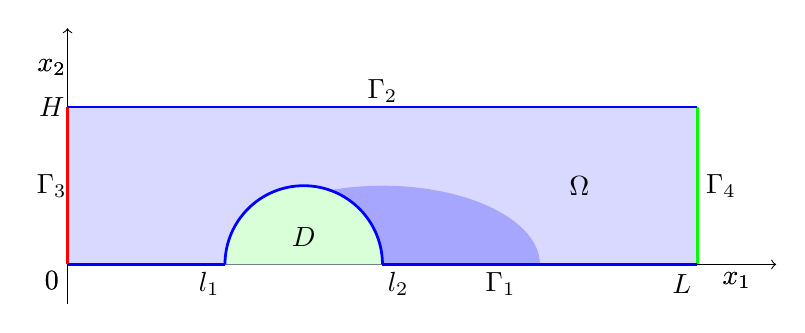
\begin{tikzpicture}
 	
 
   \fill [blue!15] (0,2) rectangle +(8.,2.);   
   
   \draw[->] (0,2) -- (9,2);
   \draw[->] (0,2-0.5) -- (0,5);
   \draw(-0.2,2-0.2) node {$0$};   
   \draw(8.5,2-0.2) node {$x_1$};   
   \draw(-0.2,4.5) node {$x_2$};     
   \draw(-0.2,4) node {$H$}; 
   
   \draw[color=red,line width=1pt] (0,2) -- (0,4);
   \draw[color=green,line width=1pt] (8,4)-- (8,2);
    
   \draw(6.5,3) node {$\Omega$};
   \draw(2-0.2,2-0.25) node {$l_1$};   
   \draw(4+0.2,2-0.25) node {$l_2$};      
   \draw(8-0.2,2-0.25) node {$L$};   

   \draw(-0.2,3) node {$\Gamma_3$};
   \draw(8.3,3) node {$\Gamma_4$};
   \draw(4.,4.2) node {$\Gamma_2$};
   \draw(5.5,2-0.25) node {$\Gamma_1$};

\draw(-0.2,2-0.2) node {$0$};   
\draw(8.5,2-0.2) node {$x_1$};   
\draw(-0.2,4.5) node {$x_2$};      

\fill [blue!35] (6,2) arc[start angle=0,end angle=180,x radius=2,y radius=1];
\fill [green!15] (4,2) arc[start angle=0,end angle=180,x radius=1,y radius=1];
\draw[color=blue,line width=1pt]  (4,2) arc[start angle=0,end angle=180,x radius=1,y radius=1];
\draw[color=blue,line width=1pt] (0,2) -- (2,2)   (4,2) -- (8,2)  (0,4) -- (8,4);

\draw(3,2.35) node {$D$};

 \end{tikzpicture}
\end{figure}


\end{document}

После: convert pdf to png
https://convertio.co/pdf-png/



 






